% 这是中国科学院大学计算机科学与技术专业《计算机组成原理(研讨课)》使用的实验报告 Latex 模板
% 本模板与 2024 年 2 月 Jun-xiong Ji 完成, 更改自由 Shing-Ho Lin 和 Jun-Xiong Ji 于 2022 年 9 月共同完成的基础物理实验模板
% 如有任何问题, 请联系: jijunxoing21@mails.ucas.ac.cn
% This is the LaTeX template for report of Experiment of Computer Organization and Design courses, based on its provided Word template. 
% This template is completed on Febrary 2024, based on the joint collabration of Shing-Ho Lin and Junxiong Ji in September 2022. 
% Adding numerous pictures and equations leads to unsatisfying experience in Word. Therefore LaTeX is better. 
% Feel free to contact me via: jijunxoing21@mails.ucas.ac.cn

\documentclass[11pt]{article}

\usepackage[a4paper]{geometry}
\geometry{left=2.0cm,right=2.0cm,top=2.5cm,bottom=2.5cm}

\usepackage{ctex} % 支持中文的LaTeX宏包
\usepackage{amsmath,amsfonts,graphicx,subfigure,amssymb,bm,amsthm,mathrsfs,mathtools,breqn} % 数学公式和符号的宏包集合
\usepackage{algorithm,algorithmicx} % 算法和伪代码
\usepackage[noend]{algpseudocode} % 算法和伪代码
\usepackage{fancyhdr} % 自定义页眉页脚
\usepackage[framemethod=TikZ]{mdframed} % 创建带边框的框架
\usepackage{fontspec} % 字体设置
\usepackage{adjustbox} % 调整盒子大小
\usepackage{fontsize} % 设置字体大小
\usepackage{tikz,xcolor} % 绘制图形和使用颜色
\usepackage{multicol} % 多栏排版
\usepackage{multirow} % 表格中合并单元格
\usepackage{pdfpages} % 插入PDF文件
\usepackage{listings} % 在文档中插入源代码
\usepackage{wrapfig} % 文字绕排图片
\usepackage{bigstrut,multirow,rotating} % 支持在表格中使用特殊命令
\usepackage{booktabs} % 创建美观的表格
\usepackage{circuitikz} % 绘制电路图
\usepackage{zhnumber} % 中文序号(用于标题)
\usepackage{tabularx} % 表格折行

\definecolor{dkgreen}{rgb}{0,0.6,0}
\definecolor{gray}{rgb}{0.5,0.5,0.5}
\definecolor{mauve}{rgb}{0.58,0,0.82}
\lstset{
  frame=tb,
  aboveskip=3mm,
  belowskip=3mm,
  showstringspaces=false,
  columns=flexible,
  framerule=1pt,
  rulecolor=\color{gray!35},
  backgroundcolor=\color{gray!5},
  basicstyle={\small\ttfamily},
  numbers=none,
  numberstyle=\tiny\color{gray},
  keywordstyle=\color{blue},
  commentstyle=\color{dkgreen},
  stringstyle=\color{mauve},
  breaklines=true,
  breakatwhitespace=true,
  tabsize=3,
}

% 轻松引用, 可以用\cref{}指令直接引用, 自动加前缀. 
% 例: 图片label为fig:1
% \cref{fig:1} => Figure.1
% \ref{fig:1}  => 1
\usepackage[capitalize]{cleveref}
% \crefname{section}{Sec.}{Secs.}
\Crefname{section}{Section}{Sections}
\Crefname{table}{Table}{Tables}
\crefname{table}{Table.}{Tabs.}

% \setmainfont{Palatino Linotype.ttf}
% \setCJKmainfont{SimHei.ttf}
% \setCJKsansfont{Songti.ttf}
% \setCJKmonofont{SimSun.ttf}
\punctstyle{kaiming}
% 偏好的几个字体, 可以根据需要自行加入字体ttf文件并调用

\renewcommand{\emph}[1]{\begin{kaishu}#1\end{kaishu}}

% 对 section 等环境的序号使用中文
\renewcommand \thesection{\zhnum{section}、}
\renewcommand \thesubsection{\arabic{section}}


%%%%%%%%%%%%%%%%%%%%%%%%%%%
%改这里可以修改实验报告表头的信息
\newcommand{\name}{艾华春, 李霄宇, 王敬华}
\newcommand{\studentNum}{2022K8009916011,2022K8009929029,2022K8009925009}
\newcommand{\major}{计算机科学与技术}
\newcommand{\labNum}{6}
\newcommand{\labName}{存储管理单元设计}
%%%%%%%%%%%%%%%%%%%%%%%%%%%

\begin{document}

\begin{center}
  \LARGE \bf 中国科学院大学 \\《计算机体系结构基础(研讨课)》实验报告
\end{center}

\begin{center}
  \emph{姓名} \underline{\makebox[10em][c]{\name}} \\
  % 如果名字比较长, 可以修改box的长度"8em"为其他值
  \emph{学号} \underline{\makebox[30em][c]{\studentNum}}\\
  % \emph{专业} \underline{\makebox[15em][c]{\major}}\\
  \emph{实验项目编号} \underline{\makebox[3em][c]{\labNum}}
  \emph{实验名称} \underline{\makebox[30em][c]{\labName}}\\
\end{center}

% \begin{center}
%   \begin{tabularx}{\textwidth}{|lX|}
%     \hline
%     注1: & 撰写此 Word 格式实验报告后以 PDF 格式保存 SERVE CloudIDE 的 \texttt{/home/serve-ide/ cod-lab/reports} 目录下(注意:reports 全部小写)。文件命名规则:\texttt{prjN.pdf},其中 \texttt{prj} 和后缀名 \texttt{pdf} 为小写,\texttt{N} 为1至4的阿拉伯数字。例如:\texttt{prj1.pdf}。PDF 文件大小应控制在 5MB 以内。此外,实验项目5包含多个选做内容,每个选做实验应提交各自的实验报告文件,文件命名规则:\texttt{prj5-projectname.pdf},其中``-''为英文标点符号的短横线。文件命名举例:\texttt{prj5-dma.pdf}。具体要求详见实验项目5讲义。 \\

%     注2: & 使用\texttt{git add}及\texttt{git commit}命令将实验报告\texttt{PDF}文件添加到本地仓库master分支,并通过\texttt{git push}推送到实验课SERVE GitLab远程仓库master分支(具体命令详见实验报告)。 \\

%     注3: & 实验报告模板下列条目仅供参考,可包含但不限定如下内容。实验报告中无需重复描述讲义中的实验流程。\\
%     \hline
%   \end{tabularx}
% \end{center}

  

\section{逻辑电路结构与仿真波形的截图及说明}
\noindent
$\bullet$
\textbf{TLB模块设计}。



\noindent
$\bullet$
\textbf{添加TLB相关指令和CSR寄存器}。
\vspace{1ex}
\begin{enumerate}
  \item 添加TLB相关指令和CSR寄存器

\item 
\end{enumerate}


\noindent
$\bullet$
\textbf{添加TLB相关例外支持,添加虚实地址映射功能}。
\vspace{1ex}
\begin{enumerate}
  \item 为cpu增加虚实映射功能
  
  在if和ex级发出访存请求的虚拟地址,同时送往直接地址翻译,直接窗口映射和tlb地址映射翻译三处,同时进行各自的
  虚实地址转换,然后再根据CSR寄存器中的值进行选择。

  以if级发出指令访存信号为例,通过组合逻辑,在同一个clk内生成三种地址翻译的结果,最后通过多路选择器进行选择。

  访存物理地址pre\_pc\_pa首先根据控制寄存器中的 crmd.pg中的值选择当前为直接地址地址翻译模式(物理地址 = 虚拟地址 = pre\_pc)
  ,还是映射地址翻译模式(物理地址 = pre\_pc\_map)。

  映射地址翻译(pre\_pc\_map)首先判断是否命中直接映射窗口,若不是,则使用tlb地址映射结构。
  
  第一行将虚拟地址 pre\_pc [31:12] 发送到tlb进行tlb地址翻译,tlb中的组合逻辑查找结果s0\_ps, s0\_ppn, s0\_found
  
  \begin{lstlisting}[language=verilog]


    assign {s0_vppn, s0_va_bit12} = pre_pc[31:12];// output to tlb
                            
    assign hit_dmw0 =           csr_dmw0_plv_met & csr_dmw0_vseg == pre_pc[31:29];
    assign hit_dmw1 =           csr_dmw1_plv_met & csr_dmw1_vseg == pre_pc[31:29];

    assign pre_pc_pa =          csr_crmd_pg ? pre_pc_map    // enable mapping
    :pre_pc;                    // direct translate

    assign pre_pc_map =  hit_dmw0 ? {csr_dmw0_pseg, pre_pc[28:0]}         // dierct map windows 0
                         :hit_dmw1? {csr_dmw1_pseg, pre_pc[28:0]}         // direct map windows 1
                         :(s0_ps == 6'b010101) ? {s0_ppn[19:9], pre_pc[20:0]}   // tlb map: ps 4Mb
                         :{s0_ppn,pre_pc[11:0]};                             // tlb map : ps 4kb
  \end{lstlisting}
  
  \item 为cpu添加tlb相关例外支持
  
  在每个流水级中设置excep\_en , excep\_ecode, excep\_esubdcode分别表示当前流水级是否触发异常,和异常的种类。

  以在ex流水级中为例:
\begin{lstlisting}[language=verilog]
  assign ex_excep_en =        ex_excep_ALE | ex_excep_TLBR|ex_excep_PIL| ex_excep_PIS| ex_excep_PPI|ex_excep_PME| id_excep_en;

  assign ex_excep_TLBR =       //TLB 重填例外
      (ex_res_from_mem | ex_mem_we) &csr_crmd_pg & ~hit_dmw0 & ~hit_dmw1 & ~s1_found;   
  assign ex_excep_PIL =       // load 操作页无效例外
      (ex_res_from_mem) &csr_crmd_pg & ~hit_dmw0 & ~hit_dmw1 & s1_found & ~s1_v;  
  assign ex_excep_PIS =       // store 操作页无效例外
      (ex_mem_we) &csr_crmd_pg & ~hit_dmw0 & ~hit_dmw1 & s1_found & ~s1_v; 
  assign ex_excep_PPI =       // 页特权等级不合规例外
      (ex_res_from_mem | ex_mem_we) & csr_crmd_pg & ~hit_dmw0 & ~hit_dmw1 & s1_found & s1_v & (s1_plv < csr_crmd_plv);
  assign ex_excep_PME =        //页修改例外
      (ex_res_from_mem | ex_mem_we) & csr_crmd_pg & ~hit_dmw0 & ~hit_dmw1 & s1_found & s1_v & (s1_plv >= csr_crmd_plv) & ~s1_d;
  
  assign ex_badv =            (id_excep_en) ? id_badv
                              : ex_alu_result;
  assign ex_esubcode =        (id_excep_en) ? id_esubcode
                              :9'b0;
  assign ex_ecode =           (id_excep_en) ? id_ecode
                              :ex_excep_ALE ? 6'h9
                              :ex_excep_TLBR ?6'h3f     // tlb refill
                              :ex_excep_PIL ?6'h1
                              :ex_excep_PIS ?6'h2
                              :ex_excep_PPI ?6'h7
                              :6'h4;  // pme
\end{lstlisting}
 所有tlb相关的异常,触发的必要条件都有:当前指令是访存指令(load/store), 当前虚拟地址翻译模式不是直接
  地址翻译模式,且不命中直接映射窗口。


  即 \verb| (ex_res_from_mem| |\verb| ex_mem_we) &csr_crmd_pg & ~hit_dmw0 & ~hit_dmw1|
  \begin{enumerate}
    \item TLB 重填例外 
    
    在tlb没有找到对应的页表项,即\verb|s1_found == 0|

    \item load 操作页无效例外, store 操作页无效例外
    
    在tlb中找到对应的页表项,但是页表项的有效位为 0, 即\verb |s1_found & ~s1_v|
    
    \item  页特权等级不合
    
    在tlb中找到对应的页表项,页表项的有效,但当前特权等级为plv3, 但是页表项所需要特权等级为plv0, 
    即 \verb|s1_found & s1_v & (s1_plv < csr_crmd_plv)|

    \item 页修改例外
    在tlb中找到对应的页表项,页表项的有效,且特权等级满足要求, 但是页表项脏位为0, 
    即 \verb|s1_found & s1_v & (s1_plv >= csr_crmd_plv) & ~s1_d|
  \end{enumerate}
  由上面的分析可知,与tlb相关的异常触发条件互斥,不用考虑不同异常间的优先级的问题。
\end{enumerate}


\section{实验过程中遇到的问题、对问题的思考过程及解决方法(比如RTL代码中出现的逻辑bug,逻辑仿真和FPGA调试过程中的难点等)}

\noindent
$\bullet$
\textbf{if级错误丢弃异常处理函数的第一条指令}。

要求在发生mmu相关异常的时候,不能向总线发出请求,所以在pre\_if级中识别到pc的虚拟地址发生异常,则将 inst\_sram\_req
拉低。

但是导致了异常传到wb级时,发出更新流水线信号flush时,将if级误判为还在等待指令返回(实际上pre\_if级没有发出请求),则
将inst_cancel信号(表示要丢弃接收到的第一条指令)拉高,导致丢弃了异常处理含数的第一条指令。
\begin{figure}[H]
  \centering
  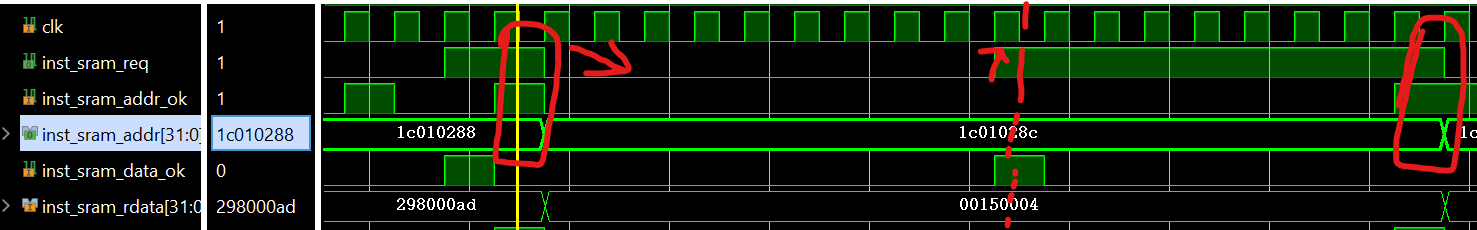
\includegraphics[width=15cm]{fig/fig1.png}
  \caption{错误拉高inst\_cancel}
\end{figure}
修改:在inst\_cancel拉高的逻辑中,判断if级是否有异常,若有,则说明if级没有已经发出请求,但是没有接受到的总线事务,
不用拉高inst\_cancel。
\begin{lstlisting}[language=verilog]
  /* 清空流水线时,第一个指令需要丢弃*/
  always @(posedge clk) begin
      if(~resetn)
          inst_cancel <= 1'b0;
      else if (   (if_valid & ~if_ir_valid & ~inst_sram_data_ok & ~if_excep_en  // if正在等待指令返回, 加入if级是否有异常的判断
                  |pre_if_reqed_reg & ~inst_sram_data_ok) // pre_if 级发出请求,但是数据没有返回,也还没有进入if级
              & (flush | br_taken))
          inst_cancel <= 1'b1;
      else if(inst_sram_data_ok)      // 异常后第一个需要被舍弃的指令返回
          inst_cancel <= 1'b0;
  end
\end{lstlisting}


      
\vspace{1ex}

\section{小组成员分工合作情况}
王敬华负责ex级访存添加类sram总线支持。

李霄宇负责部分debug工作。

艾华春负责添加TLB相关寄存器和TLB相关的例外支持,为cpu增加虚实映射功能。

实验报告为根据每人负责代码的部分,写相应部分的报告。
\end{document}